\def\year{2021}\relax
%File: formatting-instructions-latex-2021.tex
%release 2021.1
\documentclass[letterpaper]{article} % DO NOT CHANGE THIS
\usepackage{aaai21}  % DO NOT CHANGE THIS
\usepackage{times}  % DO NOT CHANGE THIS
\usepackage{helvet} % DO NOT CHANGE THIS
\usepackage{courier}  % DO NOT CHANGE THIS
\usepackage[hyphens]{url}  % DO NOT CHANGE THIS
\usepackage{graphicx} % DO NOT CHANGE THIS
\urlstyle{rm} % DO NOT CHANGE THIS
\def\UrlFont{\rm}  % DO NOT CHANGE THIS
\usepackage{natbib}  % DO NOT CHANGE THIS AND DO NOT ADD ANY OPTIONS TO IT
\usepackage{caption} % DO NOT CHANGE THIS AND DO NOT ADD ANY OPTIONS TO IT
\frenchspacing  % DO NOT CHANGE THIS
\setlength{\pdfpagewidth}{8.5in}  % DO NOT CHANGE THIS
\setlength{\pdfpageheight}{11in}  % DO NOT CHANGE THIS
\usepackage{latexsym}
\usepackage{makecell}
\usepackage{amsmath}
\usepackage{amsfonts}
\usepackage[english]{babel}
\usepackage[switch]{lineno}

%\nocopyright
%PDF Info Is REQUIRED.
% For /Author, add all authors within the parentheses, separated by commas. No accents or commands.
% For /Title, add Title in Mixed Case. No accents or commands. Retain the parentheses.
\pdfinfo{
/Title (Diverse and Specific Clarification Question Generation with Keywords)
/Author (AAAI Press Staff, Pater Patel Schneider, Sunil Issar, J. Scott Penberthy, George Ferguson, Hans Guesgen, Francisco Cruz, Marc Pujol-Gonzalez)
/TemplateVersion (2021.1)
} %Leave this
% /Title ()
% Put your actual complete title (no codes, scripts, shortcuts, or LaTeX commands) within the parentheses in mixed case
% Leave the space between \Title and the beginning parenthesis alone
% /Author ()
% Put your actual complete list of authors (no codes, scripts, shortcuts, or LaTeX commands) within the parentheses in mixed case.
% Each author should be only by a comma. If the name contains accents, remove them. If there are any LaTeX commands,
% remove them.

% DISALLOWED PACKAGES
% \usepackage{authblk} -- This package is specifically forbidden
% \usepackage{balance} -- This package is specifically forbidden
% \usepackage{color}
% \usepackage{CJK} -- This package is specifically forbidden
% \usepackage{float} -- This package is specifically forbidden
% \usepackage{flushend} -- This package is specifically forbidden
% \usepackage{fontenc} -- This package is specifically forbidden
% \usepackage{fullpage} -- This package is specifically forbidden
% \usepackage{geometry} -- This package is specifically forbidden
% \usepackage{grffile} -- This package is specifically forbidden
% \usepackage{hyperref} -- This package is specifically forbidden
% \usepackage{navigator} -- This package is specifically forbidden
% (or any other package that embeds links such as navigator or hyperref)
% \indentfirst} -- This package is specifically forbidden
% \layout} -- This package is specifically forbidden
% \multicol} -- This package is specifically forbidden
% \nameref} -- This package is specifically forbidden
% \usepackage{savetrees} -- This package is specifically forbidden
% \usepackage{setspace} -- This package is specifically forbidden
% \usepackage{stfloats} -- This package is specifically forbidden
% \usepackage{tabu} -- This package is specifically forbidden
% \usepackage{titlesec} -- This package is specifically forbidden
% \usepackage{tocbibind} -- This package is specifically forbidden
% \usepackage{ulem} -- This package is specifically forbidden
% \usepackage{wrapfig} -- This package is specifically forbidden
% DISALLOWED COMMANDS
% \nocopyright -- Your paper will not be published if you use this command
% \addtolength -- This command may not be used
% \balance -- This command may not be used
% \baselinestretch -- Your paper will not be published if you use this command
% \clearpage -- No page breaks of any kind may be used for the final version of your paper
% \columnsep -- This command may not be used
% \newpage -- No page breaks of any kind may be used for the final version of your paper
% \pagebreak -- No page breaks of any kind may be used for the final version of your paperr
% \pagestyle -- This command may not be used
% \tiny -- This is not an acceptable font size.
% \vspace{- -- No negative value may be used in proximity of a caption, figure, table, section, subsection, subsubsection, or reference
% \vskip{- -- No negative value may be used to alter spacing above or below a caption, figure, table, section, subsection, subsubsection, or reference

\setcounter{secnumdepth}{2} %May be changed to 1 or 2 if section numbers are desired.
% \newcommand{\KZ}[1]{\textcolor{blue}{Kenny: #1}}
% \newcommand{\Zl}[1]{\textcolor{blue}{Zhiling: #1}}
% The file aaai21.sty is the style file for AAAI Press
% proceedings, working notes, and technical reports.
%

% Title

% Your title must be in mixed case, not sentence case.
% That means all verbs (including short verbs like be, is, using,and go),
% nouns, adverbs, adjectives should be capitalized, including both words in hyphenated terms, while
% articles, conjunctions, and prepositions are lower case unless they
% directly follow a colon or long dash

% \title{AAAI Press Formatting Instructions \\for Authors Using \LaTeX{} --- A Guide }
% \author{

%     %Authors
%     % All authors must be in the same font size and format.
%     Written by AAAI Press Staff\textsuperscript{\rm 1}\thanks{With help from the AAAI Publications Committee.}\\
%     AAAI Style Contributions by Pater Patel Schneider,
%     Sunil Issar,  \\
%     J. Scott Penberthy,
%     George Ferguson,
%     Hans Guesgen,
%     Francisco Cruz,
%     Marc Pujol-Gonzalez
%     \\
% }
% \affiliations{
%     %Afiliations

%     \textsuperscript{\rm 1}Association for the Advancement of Artificial Intelligence\\
%     %If you have multiple authors and multiple affiliations
%     % use superscripts in text and roman font to identify them.
%     %For example,

%     % Sunil Issar, \textsuperscript{\rm 2}
%     % J. Scott Penberthy, \textsuperscript{\rm 3}
%     % George Ferguson,\textsuperscript{\rm 4}
%     % Hans Guesgen, \textsuperscript{\rm 5}.
%     % Note that the comma should be placed BEFORE the superscript for optimum readability

%     2275 East Bayshore Road, Suite 160\\
%     Palo Alto, California 94303\\
%     % email address must be in roman text type, not monospace or sans serif
%     publications21@aaai.org

%     % See more examples next
% }
% \iffalse
% %Example, Single Author, ->> remove \iffalse,\fi and place them surrounding AAAI title to use it
% \title{My Publication Title --- Single Author}
% \author {
%     % Author
%     Author Name \\
% }

% \affiliations{
%     Affiliation \\
%     Affiliation Line 2 \\
%     name@example.com
% }
% \fi

% \iffalse
%Example, Multiple Authors, ->> remove \iffalse,\fi and place them surrounding AAAI title to use it
\title{Diverse and Specific Clarification Question Generation with Keywords}
\author {
    % Authors

        First Author Name,\textsuperscript{\rm 1}
        Second Author Name, \textsuperscript{\rm 2}
        Third Author Name \textsuperscript{\rm 1} \\
}
\affiliations {
    % Affiliations
    \textsuperscript{\rm 1} Affiliation 1 \\
    \textsuperscript{\rm 2} Affiliation 2 \\
    firstAuthor@affiliation1.com, secondAuthor@affilation2.com, thirdAuthor@affiliation1.com
}
% \fi
\begin{document}
\linenumbers
\maketitle

\begin{abstract}
  Task-oriented writings like product descriptions on Amazon often suffer from the missing of important aspects. \textit{Clarification question generation} (CQGen) can be a promising approach to help alleviate the problem. Unlike traditional QGen assuming the existence of answers in the context and generating questions accordingly, CQGen mimics user behaviors of asking for unstated information. Previous works assume generating one CQ per context, but we claim that generating a group of CQs can be more beneficial by covering wider information needs. We thus propose the task of \textit{Diverse CQGen} and propose a new model named \textit{KPCNet}, which generates CQs with Keyword Prediction and Conditioning, to deal with this challenge while improving specificity at the same time. Automatic and human evaluation on 2 datasets (\texttt{Home \& Kitchen}, \texttt{Office}) showed that KPCNet can generate more specific questions and promote better group-level diversity than several competitive baselines.
\end{abstract}

\section{Introduction}
\label{sec:intro}
% \KZ{You better use section number depth 2 so the section nesting is clearly
% shown. Otherwise you yourself might be confused.}
% \Zl{Didn't notice this. Revised the references accordingly.}
The development of the Internet has spawned a number of task-oriented writings, such as product descriptions on Amazon. However, since authors cannot always have a thorough understanding of consumers' need, their writings usually miss something deemed important by the audience. For example, an American author may assume his machine be used on 110V, and thus omit this in description. Customers from 220V-using countries would pay special attention to the voltage attribute stated in the description. On finding this absent from context, some customers may ask CQs like ``What is the voltage of this machine?" in customer QA, while others would turn to other products immediately, an unfortunate loss to the seller.

\begin{figure}[htbp]
\centering
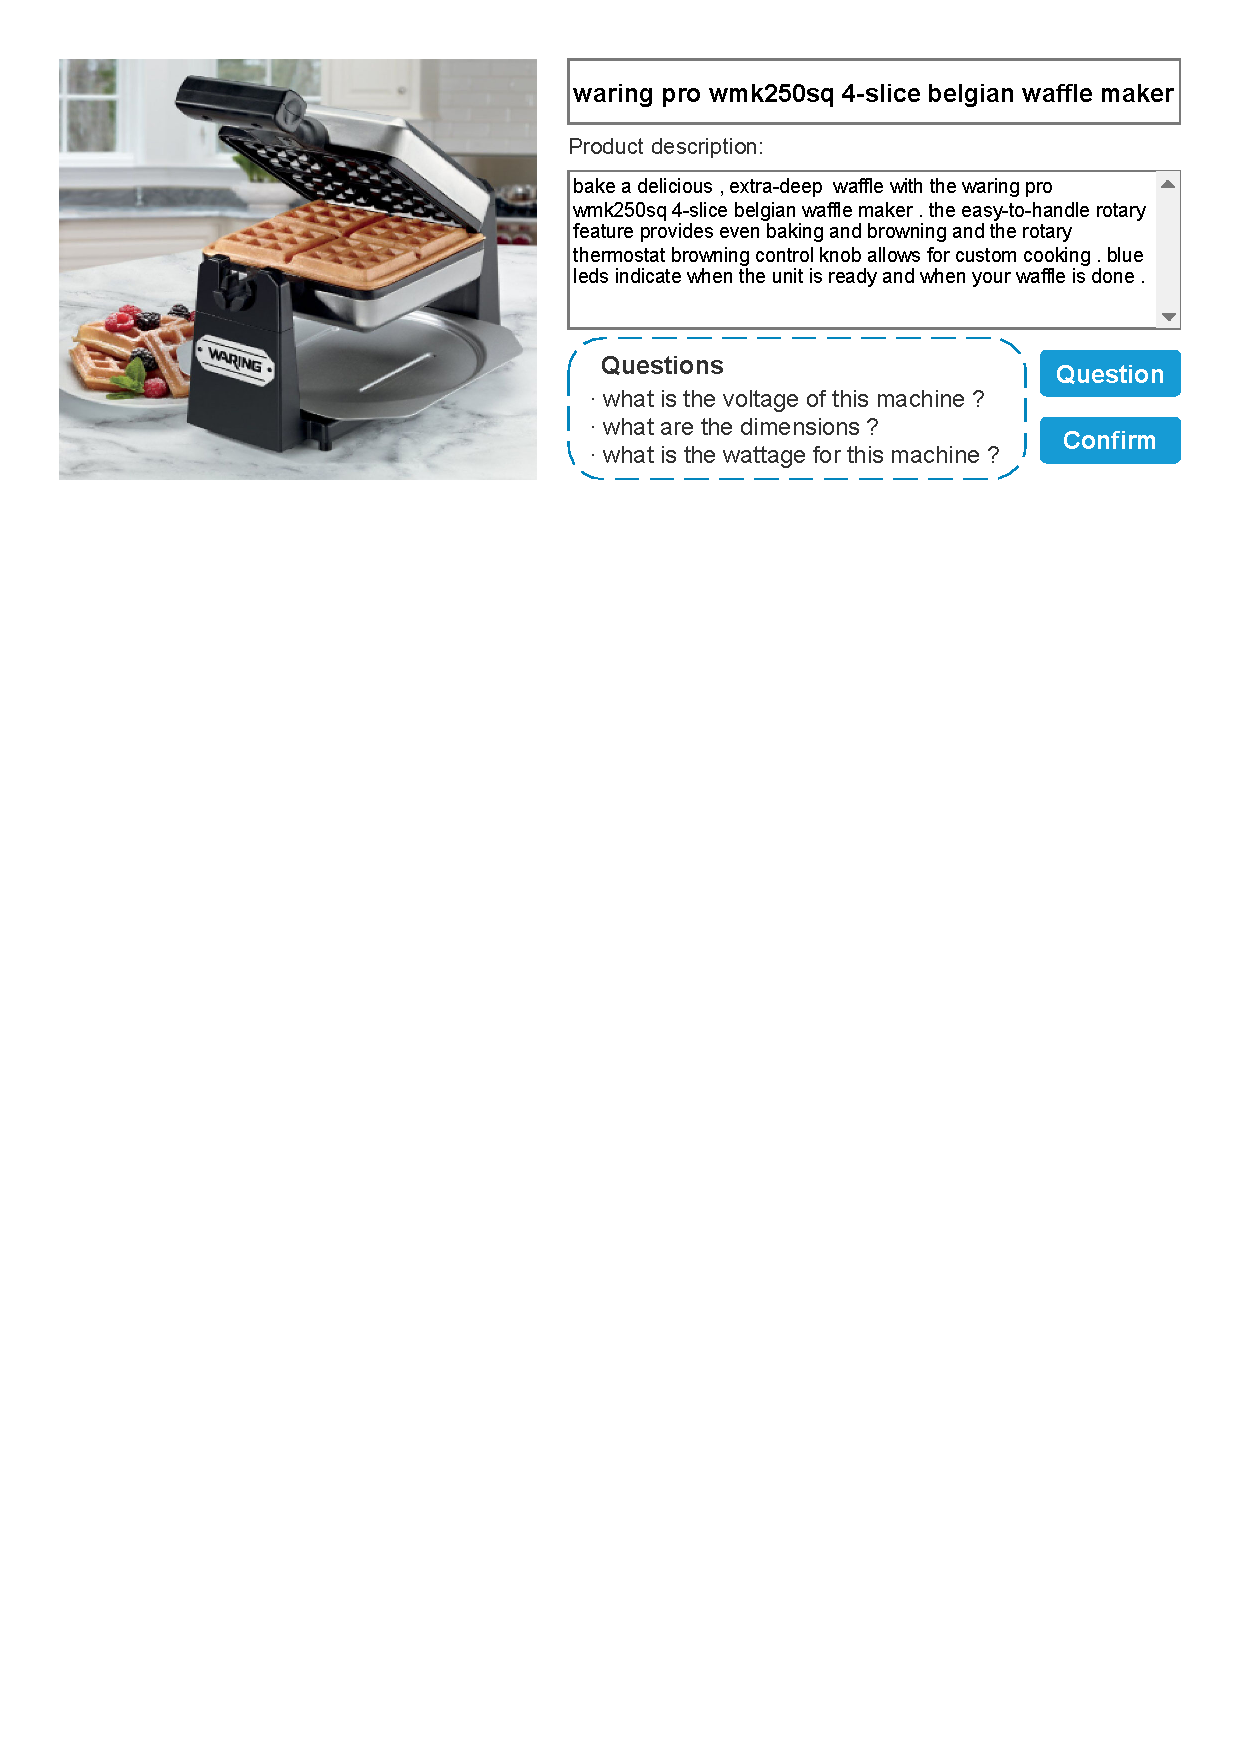
\includegraphics[width=\linewidth]{WA_UI.pdf}
\caption{A hypothetical writing assistant generating CQs.}
\label{fig:WA_UI}
\end{figure}

Clarification question\footnote{questions asking for what's missing from a given context} generation (CQGen) is a promising approach that mimics the user engagement to help alleviate the problem. Authors may request for CQs before publishing their writings from somewhere like the hypothetical writing assistant we illustrated in Figure \ref{fig:WA_UI}, and supplement missing information accordingly.

CQGen is a challenging task. First, it requires the question to be \textit{specific} while not being \textit{repetitive} to existing context. Questions with narrower application range are considered more specific. For example, the first question in Figure \ref{fig:WA_UI} is more specific than the second one because it should only be raised to electrical appliances. In contrast to the traditional QGen task which typically operates on the SQuAD 1.1 dataset \citep{rajpurkar2016squad} and derives the specificity from the knowledge of answer, CQGen doesn't expect the existence of answer in the context. Therefore, QGen algorithms which require answer and its position, either provided \citep{song2018leveraging, sun2018answer} or can be extracted \citep{subramanian2018neural}, are not applicable here. Vanilla seq2seq model has been shown to generate highly generic questions by \citet{rao2019answer}. They then proposed GAN-Utility for this problem. However, their approach requires another QA component to generate answer from context and the generated question, which may not be reliable as the answers are inherently missing from context by definition. Consequently, this approach was shown to yield even worse result under some conditions \citep{cao2019controlling}. We thus totally eliminate the involvement of answers in our work, which will also enable the gathering of training data without answer.

Moreover, previous works on CQGen all assume generating one question per context. We claim that generating a group of diversity CQs (as is shown in Figure \ref{fig:WA_UI}) can be more beneficial, because this allows the system to efficiently cover a variety of user needs at once, and become more robust to problems on any single generation. We name this novel task as \textbf{Diverse CQGen}. We seek algorithms that can deal with the task, and adopt a new group-level evaluation protocol to properly evaluate the system performance under this scenario.

To deal with the specificity challenge, we propose a novel model named Keyword Prediction and Conditioning Network (KPCNet). We observed that the main semantics of a question can be captured by its keywords. For example, the keyword of ``What's the \textit{dimension}?" is \textit{dimension}, and the question can be comprehended even with a single word (``\textit{dimension}?"). Keywords mainly consist of the product properties, and can allow for even more flexible and specific generation sometimes. For example, we can generate ``Can you cook \textit{rice} in this \textit{cooker}?" with keywords ``\textit{cooker, rice}", while it will be unsuitable to use properties to exhaust all possible ingredients like \textit{rice}. Therefore, the proposed KPCNet first predicts the probability for a keyword to appear in the generated CQ, then selects keywords from the predicted distribution, and finally conditions on them to generate questions. We can also partially control the generation by operating on the conditioned keywords, which can be utilized to avoid repetitive questions and further improve the quality.

To promote diversity, we explore several diverse generation approaches for this problem, including model-based \textit{Mixture of Experts} \citep{shen2019mixture} and decoding-based \textit{Diverse Beam Search} \citep{vijayakumar2018diverse}. KPCNet's controllability through keywords also allows keywords-based approaches. We explore a novel use of classical clustering method on producing coherent keyword groups for keyword selection to generate correct, specific and diverse questions.

Individual and group-level evaluation showed that KPCNet is capable of producing more diverse and specific questions than competitive baselines, and can thus serve as a reliable backbone of the proposed writing assistant. Our contributions are:

\begin{enumerate}
  \item We propose the task of \textit{Diverse CQGen}, which requires generating a group of diverse CQs per context, to cover a wide range of information needs. 
  \item We propose KPCNet, which first predicts keywords for specificity, and then selects keywords as the condition for generation to allow partially controllable generation.
  \item Based on the controllability of KPCNet, we propose several selection methods for conditioning keyword sets to promote diversity.
  \item We evaluate KPCNet on 2 datasets (\texttt{Home \& Kitchen} and \texttt{Office}) at both individual-level and group-level. A combination of automatic and human evaluation shows that KPCNet can achieve superior specificity in both settings and outperform strong baselines in diversity.
\end{enumerate}

\section{Preliminaries}

\subsection{Keyword-based Diverse CQGen}
Given a textual \textit{context} $x = (x_1, x_2, ..., x_{T_1})$, our aim is to generate a \textit{clarification question} $y = (y_1, y_2, ..., y_{T_2})$, so that $y$ asks for relevant but not repetitive information to $x$. In the setting of \textit{Diverse CQGen}, we should generate a group of CQs for the same context such that they are semantically different from each other. In this work, we additionally consider \textit{keywords} $Z = (z_1, z_2, ..., z_k)$ that are expected to capture the main semantic of $y$. Here we define keywords as lemmatized, non-stopping nouns, verbs and adjectives appearing in \textit{questions}. Note that keywords are different from \textit{answers}, and we don't assume the existence of answer in our approach. We extract a keyword dictionary $\mathcal{Z}$ of size $C$ from the training set using this definition. 

With keywords introduced, the marginal likelihood of a question are decomposed as:

\begin{equation}
  \begin{split}
    p(y|x) &= \sum_{Z \subseteq \mathcal{Z}}p(y, Z|x) \\ 
    &= \sum_{Z \subseteq \mathcal{Z}}p(y|x,Z)p(Z|x)
  \end{split}
  \label{equ:decompose}
\end{equation}

\subsection{Specificity}
\label{sec:specific}
In this work, the specificity of a question is determined with the size of its applicable range. Question that can only be raised against one particular context is considered more specific than universal questions. Firstly, \textit{relevance} is the basic requirement of specificity. Traditional MLE training may generate generic but not relevant question for higher likelihood. We hypothesize that the additional task of keyword prediction will help focus on relevant aspects. Besides, \textit{specificity} of e-commerce questions are further promoted in 3 ways according to our observation : (1) Focusing on certain aspects, like the type, brand and attributes. (2) Mentioning components of a product, e.g. blade of a food grinder. (3) Describing a using experience specific to the product, such as cooking rice in a cooker. We hypothesize that many of them can be captured by keywords, with nouns and adjectives covering aspects and components, and verbs constituting the using experience.

\subsection{Diversity}

Diverse CQGen requires a group of questions to be generated about the same context, to cover various information needs as well as improve the robustness to problematic generations. This setting differs from some previous literatures \citep{wang2018learning, rao2019answer}, where we generate only one response at a time, and \textit{Diversity} is used to measure the expected variety of content and patterns among \textit{all generated response}. We call it \textit{global diversity}. Our setting is referred to as \textit{local diversity}, measuring the diversity \textit{within one usage}. This is also adopted by another line of literatures \citep{vijayakumar2018diverse, shen2019mixture}. If not specified, we mean \textit{local diversity} by using \textit{diversity}. Global diversity is also desired, as it increases the likelihood of the questions to be specific to various contexts. 

To meet the diversity requirement as well as to promote specificity, we propose KPCNet below.


\section{Model Description}
\label{sec:KPCNet}
In Equation \ref{equ:decompose}, $p(Z|x)$ corresponds to the keyword prediction part, and $p(y|x,Z)$ refers to the keyword conditioned generation. Our model is thus divided into 2 logical parts. The whole model pipeline is illustrated in Figure \ref{fig:pipeline}. 


\begin{figure}[htbp]
  \centering
  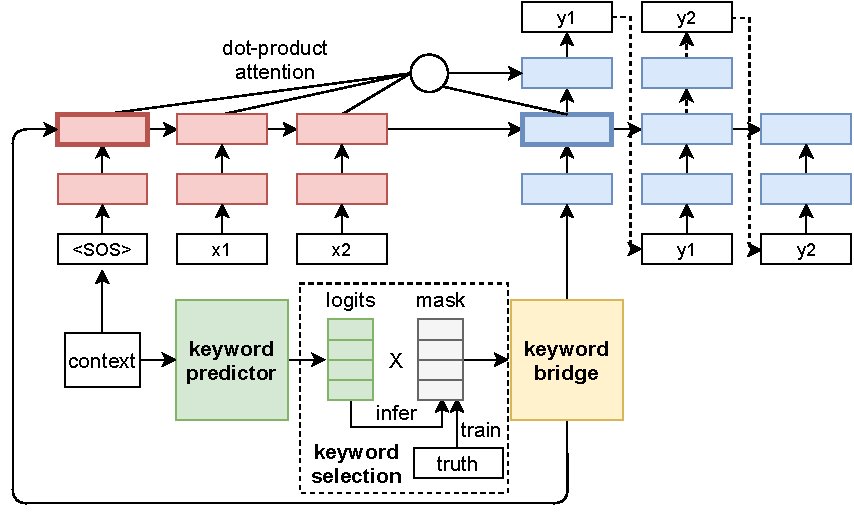
\includegraphics[width=1\linewidth]{kwd_model.pdf}
  \caption{Illustration of KPCNet.}
  \label{fig:pipeline}
  \end{figure}

\subsection{Keyword Prediction}

For the \textit{Keyword Predictor}, we assume the probability of each keyword $z$ are independent from each other given context $x$, i.e. $p(Z|x)=\Pi_{z \subset Z}p(z|x)$, to simplify the modeling. We parameterize $p(z|x)$ with TextCNN \citep{kim-2014-convolutional}. The training loss is binary cross entropy over each keyword:

\begin{equation}
  L_{pred} = -\frac{1}{N}\sum_{n=1}^{N}\sum_{c=1}^{C}z^t_{n,c}log(p_{n,c})
  \label{equ:pred}
\end{equation}
$z^t_{n,c}$ is a binary indicator shows if keyword $c$ is among the ground truth keywords of the $n_{th}$ sample, and $p_{n,c}$ is the predicted probability for $c$.

\subsection{Keyword Conditioned Generation}

The main structure of our generator is based on a standard sequence-to-sequence model \citep{luong2015effective}. We will focus on our specific design to condition the generation on keywords. 

\paragraph{Keyword Selection} We take the unnormalized keyword logits $\hat{p} \in \mathbb{R}^C$ from the keyword predictor, and then we select a conditioning keyword set $Z^s$ to mask out irrelevant dimensions to get a masked logits $\tilde{p} = [\hat{p}_1 z^s_1, \hat{p}_2 z^s_2, ..., \hat{p}_C z^s_C]$. This procedure allows us to control the generation with the selected keywords. Specific methods for this part will be discussed in Sec \ref{sec:selection}.

\paragraph{Keyword Bridge} After getting the masked logits $\tilde{p}$, we pass them through a dropout layer, and then transform them to another distributed representation using a Multi-Layer Perceptron (MLP). They are then transformed into encoder features and decoder features with 2 MLPs respectively. The encoder feature will replace the hidden state of the first encoder step as memory to guide the generation via attention. The decoder feature will be fed as the input word embedding of the first decoder step to influence the generation.

\subsection{Keyword Selection}
\label{sec:selection}
% \KZ{What's the logical relation between this subsection and 
% paragraph ``keyword selection'' above?}
% \Zl{This part details the sketch above, forward reference added.}
At training, the ground truth keywords set $Z^t$ is selected as $Z^s$, and the training objective is to maximize the log-likelihood of all questions given context $x$ and keywords $Z^t$. This equals to minimize: 

\begin{equation}
  L_{mle} = -\frac{1}{N}\sum^N_{n=1}log(p(y_n|x_n,Z^t_n))
  \label{equ:mle}
\end{equation}

At inference, we select $Z^s$ from keyword predictor's predicted distribution as condition for generation. This process was done once at a time, and can be done several times to fully explore the diversity in $p(y|x)$ with different keyword sets. We come up with 3 methods for keyword selection:

\paragraph{Threshold} We select all keywords whose predicted probability is above a threshold $\alpha$ as $Z^s$. If not specified, this is the default selection method at inference.

\paragraph{Sampling} The threshold selection approach is deterministic and thus limited to one conditioning keyword set. We may encourage more diverse generation via diversifying the keyword set. An intuitive solution is to introduce randomness. Inspired by the Top-K \citep{fan-etal-2018-hierarchical, radford2019language} and Top-p (nucleus) sampling \citep{holtzman2019curious}, we also adopted a similar approach, sampling $k$ keywords from softmax-normalized prediction distribution after Top-K, Top-p filtering.

\paragraph{Clustering} Both of the threshold and sampling selection strategy run the risk of putting semantically uncoherent keywords together, which is the drawback of the independence assumption used by keyword predictor. For example, if \textit{``voltage, machine, long, waffle"} are selected as the keywords for the waffle maker in Figure \ref{fig:WA_UI}, we may generate an illogical question ``what are the \textit{voltage} of the \textit{waffle}". To get more coherent keyword sets, we explore the use of clustering technique. For the above example, the keywords can form 2 semantic groups, which lead to ``What are the \textit{voltage} of the \textit{machine}" and ``How \textit{long} does it take to cook \textit{waffle}", respectively. 

In practice, we first mine a keyword co-occurrence graph from the training set. We then take the Top-K likely keywords, and run Spectral clustering \citep{Shi00normalizedcuts} on the induced subgraph of them. The resulting $g$ disjoint groups are then used as generation conditions respectively.

\subsubsection{Keyword Controllability Probing}

One potential benefit that KPCNet brought is the controllability over generation by providing different conditioning keywords. To probe into this, we propose 2 approaches to operate on the keywords besides the 3 keywords selection methods. The operations are designed with hypotheses that will be tested with experiments.

\begin{table}
  \small
  \centering
\begin{tabular}{l|l}
\hline
Product & \makecell[l]{iliving organic buckwheat pillow with authentic \\ japanese pillow cover, 14 by 20-inch, green } \\
\hline
KPCNet & \makecell[l]{what is the \textbf{size} of this \textbf{pillow} case? \\ (size, cover, pillow, wash, zipper)} \\
+Filter        & \makecell[l]{does this \textbf{pillow} have a \textbf{zipper}? \\ (cover, pillow, wash, zipper)} \\
\hline
\end{tabular}
\caption{\label{tab:kwd-filter} Example on the effect of keyword filtering. Predicted keywords for a question are shown in the parentheses below. ``size" was filtered as it has already been covered in product description.}
\end{table}

\paragraph{Keyword Filtering} \label{para:filter} Avoiding to ask existing information in the context is the basic requirement of CQ. However, none of existing methods in the literature proposed a specific approach to tackle this. In preliminary experiments of KPCNet, we found that some of the repetitive cases came with repetitive keywords. Therefore, we conjecture that we may alleviate the problem by filtering out such repetitive keywords. Table \ref{tab:kwd-filter} provided a concrete example. This would be especially useful for iterative generation, as we will explicitly exclude repeating keywords if user triggers CQGen for the second time with some information vacancy already filled.

Here we use a simple matching method for keyword filtering. We first select a set of keywords that tends to lead to repetition. Then for each keyword in the set, we write a blacklist of words or patterns so that we filter the keyword if the pattern is matched. This process is currently done manually, so it doesn't scale. However, we find that a small set of frequent keywords is already enough to cover a relatively large number of repetitive cases and demonstrate the effect of this approach. We leave automatic repeating keyword detection and filtering for future works.  

\paragraph{External Knowledge} \label{sec:knowledge} It is a common practice for e-commerce platforms to build knowledge graph to manage their products \citep{dong2018challenges, luo2020alicoco}. As a result, products are attached to highly related tags, concepts, or keywords in our terms. We hypothesize that such external knowledge may help the generation by directly providing high-quality keywords, or improving the keyword prediction. Nevertheless, since we don't have access to such knowledge, we simulate such scenario where we have higher quality keywords by directly feeding ground truth keywords to the model[KPCNet(truth)]. This establishes an upper bound to what extent can KPCNet be improved with knowledge.

\subsection{Deduplication Postprocessing}
\label{sec:deduplicate}
All algorithms will more or less produce semantically similar questions in their initial generation group. Therefore, we will first generate more candidates than needed (say, produce 6 questions for 3 displaying slots), so that at least certain level of diversity can be guaranteed for the initial group. We then apply a simple, model-agnostic heuristic for deduplicating question selection. We first add the top generation into the current group, then we will iterative through the remaining questions. If the question's Jaccard similarity with any currently selected question is below 0.5, it will be added into the current group, otherwise it will be skipped. 

\section{Experiments}
\label{sec:experiments}
The research problems we want to tackle here are: 
(1) Can KPCNet generate more specific CQs? 
(2) To what extent can we control the generation of KPCNet by operating on the keywords? 
(3) How well can our proposed keyword selection methods promote local diversity, compared to existing diverse generation approaches?

\subsection{Evaluation metrics}
Most previous works on question generation \citep{jain2017creativity, hu2018aspect, rao2019answer} adopts \textit{Individual-level} evaluation protocol, where only the best generated question of a group is evaluated (thus also named \textit{Oracle} metrics). Specially, for proper evaluation of the novel \textit{Diverse CQGen} task, we need to evaluate the overall quality and diversity of CQ groups. We refer to this as \textit{Group-level} evaluation. We adopt automatic metrics as well as human judgements on both level. 

\subsubsection{Automatic Metrics}
We use \textbf{Distinct-3} (DIVERSITY), \textbf{BLEU}\footnote{\url{https://github.com/moses-smt/mosesdecoder/blob/master/scripts/generic/multi-bleu.perl}}\citep{papineni2002bleu} and 
\textbf{METEOR} \citep{banerjee2005meteor} for individual-level automatic evaluation.

For group-level evaluation, we adopt the evaluation protocol proposed by \citet{shen2019mixture} for diverse machine translation, and use \textbf{Pairwise-BLEU} and \textbf{Avg BLEU} as the evaluation metric.
% \KZ{Instead of showing the pairwise bleu score in the fig, I'd rather see more
% example generated questions for both datasets. For generation tasks, audience
% are more interested in eyeballing the results and see some analysis of the
% results than looking at dry numbers! Give analysis, analysis, analysis!}
% \Zl{Due to space limit, more examples provided in Appendix.}
\subsubsection{Human Judgements}
For individual-level human judgements, we show the annotator one context and one generated question for each system (including reference). The system name is invisible to the annotator and the order is randomly shuffled. The selected candidate is the one that achieved the highest BLEU in the generation group. 

We ask human to judge the \textbf{Grammaticality(G), Relevance(R), Seeking New Information(N) and Specificity(S)} of the questions. Also, noting that the system generations are also prone to make logical errors like improper repetition (``does the lid have a lid ?") or asking for relevant but not exactly the correct object (asking ``what is the thickness of the bed ?" for a mattress), we further judge the \textbf{Logicality(L)} of the candidate.

For group-level human judgements, we run the deduplication procedure (Sec \ref{sec:deduplicate}) to get 3 top questions for each system. And annotators are showed one context and the selected 3 questions for every group. The groups are also anonymized and shuffled.

For each question in a group, we score the same metrics as those for individual-level judgements. To evaluate the valid variety of each group produced by local generation diversity, we introduced an additional and important group-specific metric: \textbf{\#Useful}. This is the number of useful questions after excluding problematic (ungrammatical, irrelevant, illogical, etc.) and semantically equivalent questions within a group. And we further calculate \textbf{\#Redundant} as (the number of unproblematic questions - \textbf{\#Useful}) to measure local redundancy.

Individual-level and group-level evaluation was conducted on the same set of 100 sample products for 8 systems and every group has 3 questions. They are distributed to 4 annotators so that each of the 2400 questions are annotated twice. We report inter-annotator agreement in Appendix.

\subsection{Dataset}
We evaluate our model on the \texttt{Home \& Kitchen} category of the Amazon Dataset preprocessed by \citet{rao2019answer}. We applied extra preprocessing on the raw data to remove noises in dataset (see Appendix). In this dataset, \textit{context} is the product title concatenated with the product description, and \textit{question} is the CQ asked by customers to the product. It consists of 19,119 training, 2,435 validation and 2,305 test examples (product descriptions), with 3 to 10 questions (average: 7) per description. The inherent diversity of questions in the dataset allows the proper evaluation of group-level generation diversity. We processed another category, \texttt{Office}, in a similar way. This is a much smaller dataset, consisting of 2,190 training, 285 validation and 256 test examples, with 3 to 10 questions (average: 6) per description. We will first analyze the results on \texttt{Home \& Kitchen} in detail, then briefly discuss the results on \texttt{Office}.

\subsection{Baselines}

For individual-level generation, we compare KPCNet with the following models: \textbf{MLE} Vanilla seq2seq model trained on (context, question) pairs using maximum likelihood objective.  \textbf{hMup} A representative of the family of mixture models proposed in \citet{shen2019mixture}, which achieved a good balance of overall quality and diversity. Since we don't assume the availability of answers, we don't include traditional QGen methods and GAN-Utility \citep{rao2019answer} in the comparison.

For a fair comparison, we control the encoder and decoder for all the above methods to have a similar 2-layer GRU \citep{cho2014learning} or LSTM \citep{hochreiter1997long} architecture and close amount of parameters. 

For group-level generation, we compare across 3 categories of diverse generation methods:

\paragraph{Decoding based} Classical beam search naturally produces different generation on each beam. Therefore, we evaluate the effect of beam search combined with MLE and KPCNet with threshold selection [KPCNet(beam)]. Recently, several decoding approaches \citep{ippolito2019comparison} are proposed to further promote diversity in generation, among which \textit{Diverse Beam Search}\citep{vijayakumar2018diverse} and \textit{Biased Sampling} like top-K, top-p sampling \citep{fan-etal-2018-hierarchical, holtzman2019curious} are representative methods. So we also evaluate KPCNet with them [KPCNet(divbeam), KPCNet(BSP)].

\paragraph{Model based} hMup is designed for diversity at the model level. It provides a discrete latent variable called \textit{expert} to control the generation. We thus take the top beam-searched candidate of each expert to form a generation group for evaluation.

\paragraph{Keywords based} This is dedicated to KPCNet. We evaluate the \textit{Sampling}[KPCNet(sample)] and \textit{Clustering}[KPCNet(cluster)] methods for keyword selection. We also estimate the potential of KPCNet with knowledge (Sec \ref{sec:knowledge}) by providing the ground truth keyword set [KPCNet(truth)].

All systems using beam search have a beam size of 6, we also set number of experts for hMup to 6, and we use beam size of 6 with 3 diverse groups for \textit{diverse beam search}. We select 2 keyword groups for KPCNet(sample) and KPCNet(cluster). To produce the final generation group for evaluation, outputs of all systems will go through the same deduplication postprocessing (Sec \ref{sec:deduplicate}) to get 3 questions for each group.

\subsection{\texttt{Home \& Kitchen} Dataset Results}

\subsubsection{Individual-level Evaluation}

Table \ref{tab:ind-auto-eval} shows the automatic evaluation results. KPCNet and hMup outperform MLE in METEOR but not in BLEU. We claim that it is due to the shorter and the safer generation of MLE, which is naturally favored by precision-based BLEU but not F-based METEOR. The average generation length is 5.957 for MLE, 8.231 for hMup, and 7.263 for KPCNet. KPCNet significantly outperform all the other baselines in Distinct-3 and METEOR, showing that KPCNet potentially promote higher global diversity and generation quality. We note that KPCNet(truth) has a great advantage over KPCNet, indicating the controllability of keywords and the potential of KPCNet to be further strengthened by improving the conditioned keyword set with other helpers like external knowledge (Sec \ref{sec:knowledge}).

\begin{table}[h]
  \small
  \centering
  \begin{tabular}{l|ccccc}
  \hline
  {} & Distinct-3 & BLEU & METEOR \\
  \hline
  ref  &        0.6934 &        - &    - \\
  \hline
  MLE &        0.0777 &  \textbf{18.13} & 14.86 \\
  hMup &        0.1111 &  17.76 &    15.40  \\
  KPCNet &        \textbf{0.1530} &     17.77 &    \textbf{16.18}  \\
  \hline
  KPCNet(truth) &        0.3738 &     23.63 &    19.38  \\
  \hline
  \end{tabular}
  \caption{\label{tab:ind-auto-eval} Individual-level automatic evaluation results on \texttt{Home \& Kitchen} dataset.}
\end{table}

\begin{table}[bp]
  \small
  \centering
  \begin{tabular}{l|ccccc}
  \hline
  {} & G & R & L & N & S \\
  \hline
  ref  &        0.98 &        1.00 &    1.00 &     0.94 &     2.68 \\
  \hline
  MLE  &        \textbf{0.99} &     0.92 &    \textbf{0.98} &     \textbf{0.85} &     1.45 \\
  hMup &        \textbf{0.99} &     0.92 &    0.86 &     0.81 &     1.81 \\
  KPCNet &        \textbf{0.99} &     \textbf{0.99} &    0.95 &     0.80 &     1.81 \\
  KPCNet(filter) &        \textbf{0.99} &     \textbf{0.99} &    0.94 &     \textbf{0.85} &     \textbf{1.84} \\
  \hline
  \end{tabular}
  \caption{\label{tab:ind-human-eval} Individual-level human evaluation metrics on 100 sample products from \texttt{Home \& Kitchen}. G/R/L/N/S stand for Grammatical, Relevance, Logicality, New Info and Specificity respectively.}
\end{table}



\begin{table*}[htbp]
  \centering
  \small
  \begin{tabular}{l|ccccccc}
    \hline
    {} & Relevant\tiny{[0-1]} & Logical\tiny{[0-1]} & New Info\tiny{[0-1]} & Specific\tiny{[0-4]} & \#Useful\tiny{[0-3]} & \#Redundant\tiny{[0-2]} & Avg Rank \\
    \hline
    ref          &    0.990 &   1.000 &    0.947 &    2.530 &   2.680 &      0.120 & - \\
    \hline
    MLE          &    0.907 &   \textbf{0.943} &    \textbf{0.863} &    1.457 &   1.550 &      0.590 & 3.667 \\
    hMup         &    0.900 &   0.793 &    0.833 &    1.727 &   1.530 &     \textbf{0.130} & 4.667 \\
    \hline
    KPCNet(-filter)  &    \underline{\textbf{0.987}} &   \underline{0.870} &    \underline{0.830} &    1.757 &   1.280 &      0.750 & 4.500 \\
    KPCNet(beam)    &    \underline{\textbf{0.987}} &   \underline{0.853} &    \underline{\textbf{0.863}} &    1.793 &   1.330 &      0.750 & 3.667 \\
    KPCNet(divbeam) &    \underline{0.963} &   0.780 &    \underline{0.860} &    1.760 &   1.480 &  \underline{0.310} & 4.167 \\
    KPCNet(sample)  &    \underline{0.963} &   \underline{0.837} &    \underline{0.850} &    \underline{\textbf{1.890}} &   1.500 &      0.450 & 3.500 \\
    KPCNet(cluster)  &    \underline{0.963} &   \underline{0.863} &    \underline{0.823} &    \underline{1.877} &   \underline{\textbf{1.760}} &      \underline{0.190} & \textbf{3.000} \\
    \hline
    \end{tabular}
  \caption{\label{tab:group-human-eval} Group-level human evaluation results on 100 sample products (300 questions each system) from \texttt{Home \& Kitchen}. Grammatical is omitted as the results are similar to Table \ref{tab:ind-human-eval} where all systems performs well. \textit{Avg Rank} is the average ranking among all 7 methods across the 6 metrics. We perform hypothesis test among KPCNet variants, and the difference between underlined and non-underlined numbers at each column is statistically significant with $p \leq 0.05$.}
  \end{table*}


Table \ref{tab:ind-human-eval} shows the individual-level human evaluation results. We can see that all systems perform well in \textit{Grammatical}, KPCNet significantly outperform other systems in \textit{Relevant} and achieved the best \textit{Specific}, while perform slightly worse in \textit{Logical}. The superior \textit{Relevant} proves our hypothesis that independently trained keyword predictor help focus on relevant keywords instead of irrelevant but generic words preferred by MLE (Sec \ref{sec:specific}). KPCNet(filter) gets a much higher \textit{New Info} at the cost of only slight drop in \textit{Logical}. This shows that the Keyword Filtering step (Sec \ref{para:filter}) can truly utilize the controllability of keywords to help avoid repetition. Therefore, we by default incorporate the step with all the KPCNet variants in the next group-level evaluation stage while keep the plain KPCNet for comparison as KPCNet(-filter).

\subsubsection{Group-level Evaluation}

  \begin{figure}[htbp]
    \centering
    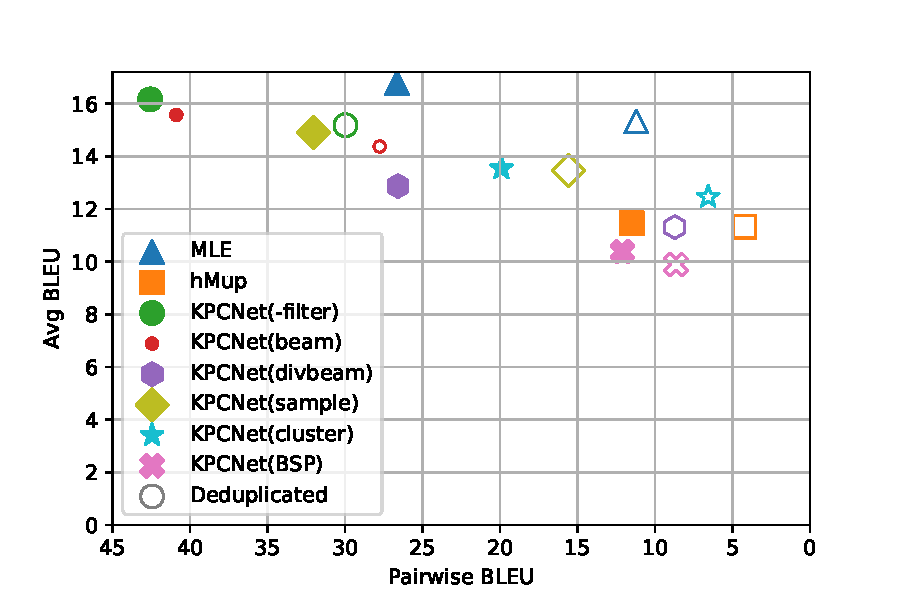
\includegraphics[width=\linewidth]{tradeoff-2BLEU.pdf}
    \caption{Group-level Automatic metrics on the whole test set of \texttt{Home \& Kitchen}. The lower Pairwise BLEU, the more diverse for the generation group. Solid markers are the results for the top 3 candidates in the original group, while hollow markers measures the remaining 3 after deduplication. Points located near top-right are preferred as they achieve a good tradeoff between the 2 metrics.}
    \label{fig:group-filter}
    \end{figure}


The group-level automatic evaluation metrics before and after deduplication for each system are shown in Figure \ref{fig:group-filter}. Original results are shown in solid markers. KPCNet(BSP) has the poorest Avg BLEU and we found the results very likely to be ungrammatical and illogical, and we thus omit it in later judgements. hMup has the highest local diversity while has the second poorest Avg BLEU. MLE has moderate level of local diversity and the highest Avg BLEU, and we found that Keyword Filtering slightly harmed Avg BLEU, which is against our intuition. But we later found Avg BLEU doesn't correlate well with most human judgements (see Appendix). Several diversity-promoting variants of KPCNet improved local diversity at the cost of Avg BLEU, among which KPCNet(cluster) achieved a best tradeoff between the two. Comparing the original and deduplicated results (hollow markers), we can see that our simple heuristic can effectively eliminate redundancy at the cost of slight degradation of Avg BLEU, as only nearly identical hypotheses with high BLEU are excluded. 

Group-level human evaluation results are shown in Table \ref{tab:group-human-eval}. We can see that all KPCNet variants clearly outperform baselines in \textit{Relevant} and \textit{Specific} while have a competitive performance in \textit{New info}. MLE rated best for \textit{Logical} for its conservative generations (low \textit{Specific}), and the questions tend to overlap with each other, as is reflected in high \textit{\#Redundant}. KPCNet(beam) has a even higher redundancy since its searching space is further limited by the conditioned keyword set. Diverse generation variants can help overcome this drawback. Especially, KPCNet(cluster) achieved the best \textit{\#Useful}, \textit{Avg Rank}, and its performance on all metrics is among the best of KPCNet variants. This shows that the semantically-coherent keyword sets produced by clustering can effectively improve the generation diversity and quality of KPCNet. 

\subsubsection{Case Study}
\begin{table}[h]
  \small
  \centering
  \begin{tabular}{l|l}
  \hline
  Product & \makecell[l]{Novaform memory foam comfort curve pillow} \\
  \hline
  \makecell[l]{KPCNet \\ (cluster)} & \makecell[l]{is this a \textbf{firm} \textbf{pillow}? (pillow, foam, sleep, firm) \\ is this pillow good for \textbf{stomach sleepers}? \\ (stomach, sleeper)} \\
  \hline
  Product & \makecell[l]{full-sized headboard in solid wood} \\
  \hline
  \makecell[l]{KPCNet \\ (cluster)} & \makecell[l]{what is the height of this \textbf{headboard} ? \\ (bed frame headboard) \\ does it have a \textbf{box spring} ? (mattress box spring)} \\
  \hline
  \end{tabular}
  \caption{\label{tab:kwd-cluster} Example generation groups for KPCNet(cluster). Keywords in the parentheses.}
  \end{table}

  

\begin{table*}[htbp]
  \centering
  \small
  \begin{tabular}{l|ccccccc}
  \hline
  {} & Grammatical\tiny{[0-1]} & Relevant\tiny{[0-1]} & Logical\tiny{[0-1]} & New Info\tiny{[0-1]} & Specific\tiny{[0-4]} & \#Useful\tiny{[0-3]} & \#Redundant\tiny{[0-2]} \\
  \hline
  ref         &       0.993 &    0.997 &   0.993 &    0.933 &    2.713 &   2.420 &      0.330 \\
  \hline
  MLE         &       0.970 &    0.843 &   \textbf{0.883} &    0.797 &    1.470 &   1.070 &      0.420 \\
  KPCNet &       \textbf{0.993} &    \textbf{0.940} &   0.817 &    \textbf{0.803} &    \textbf{1.903} &   \textbf{1.470} &      \textbf{0.190} \\
  \hline
  \end{tabular}
  \caption{\label{tab:group-human-eval-office} Group-level human judgments on 100 samples from the \texttt{Office} dataset. KPCNet here uses keyword clustering.}
\end{table*}


Table \ref{tab:kwd-cluster} provided 2 example generation groups of KPCNet(cluster). For each group, the 6 predicted keywords captured specific aspects of the product. Then they are divided into 2 coherent groups (as they formed natural phrases such as ``firm pillow'' and ``stomach sleeper'') by clustering. Finally, the different conditioned keyword sets are reflected in the generation. In the first case, specific and diverse generations are successfully produced with precisely predicted keywords. We can see that the separation of keywords as controlling factors allows the novel use of classical clustering technique to help generate high-quality question groups by first producing coherent keyword sets. There are also bad cases like the second question in another group. The possible reason is that keyword predictor produced related but unsuitable keywords ``box spring'', which can be asked for a whole bed but not for headboard alone. This shows that predictor is the performance bottleneck of KPCNet. We provide an example of group-level human judgement results including all systems in Appendix.

\subsection{\texttt{Office} Dataset Results}


\begin{table}[h]
  \centering
  \small
  \begin{tabular}{l|ccccc}
  \hline
  {} & Distinct-3 & BLEU & METEOR \\
  \hline
  ref  &        0.7554 &        - &    - \\
  \hline
  MLE &        0.2033 &  \textbf{14.73} & 13.81 \\
  hMup &        0.1531 &  10.45 &    12.52  \\
  KPCNet &        \textbf{0.3099} &     13.84 &    \textbf{15.29}  \\
  \hline
  \end{tabular}
  \caption{\label{tab:ind-auto-eval-office} Individual-level automatic evaluation results on the \texttt{Office} dataset.}
\end{table}

For brevity, we only show the individual-level automatic evaluation and group-level human judgement results. All the experimental settings are the same with the previous experiments, except that we apply no keyword filtering here. 

Table \ref{tab:ind-auto-eval-office} shows that KPCNet still outperforms MLE in Distinct-3 and METEOR, while falls behind at BLEU. Both the automatic metrics and our manual check indicate that hMup fails to give comparable performance at the small dataset, so we exclude it in group-level evaluation. 

Table \ref{tab:group-human-eval-office} showed that the performance of both models degraded here possibly due to the smaller data size. However, the observation is similar. KPCNet(cluster) outperforms MLE in most metrics especially at \textit{Relevant}, \textit{Specific} and \textit{\#Useful} despite a weakness at \textit{Logical}. This shows that KPCNet(cluster) can consistently improve the diversity and specificity of the generation.


\section{Related Work}
\paragraph{Clarification Question Generation} The concept of CQ can be naturally raised in a dialogue system for incomplete recognition \citep{stoyanchev2014towards} or task-oriented slot-filling. The concept is then extended to IR to clarify ambiguous queries \citep{aliannejadi2019asking}, and has been successfully put into practice \citep{Zamani2020GeneratingCQ}. Our work closely follows the research line of \citet{rao2018learning, rao2019answer, cao2019controlling}, which sets the problem in the task-oriented writing scenario. \citet{rao2018learning} first adopted a retrieval-then-rank approach, \citet{rao2019answer} then proposed a generation approach to train the model to maximize the utility of the hypothetical answer for the questions with GAN, to better promote specificity. \citet{cao2019controlling} propose to control the specificity by training on data with explicit indicator of specificity, but it requires additional specificity annotation. Towards the similar specificity goal, we adopted a different keyword-based approach. Parallel to our work, \citet{Kumar_2020} proposed ClarQ, a large-scale and diverse dataset for CQGen derived from StackExchange.

\paragraph{Diverse Generation} The demand for diverse generation exists in many other fields, and we've drawn inspirations from these literatures. For image captioning, we may use multiple descriptions for different focusing points of a scene. \textit{Diverse Beam Search} \citep{vijayakumar2018diverse} was proposed to broaden the searching space to catch such diversity by dividing groups in decoding and imposing repetition penalty between them. For machine translation, a context can be translated with different styles. \citet{shen2019mixture} thus proposed \textit{Mixture of Expert} models including hMup to reflect various styles with a discrete latent variable (\textit{expert}). And here for CQGen, diversity is required to cover various potentially missing aspects, so we come up with the idea to use keywords as a controlling variable  like \textit{expert} to promote diversity.

\section{Conclusion}
We propose the task of Diverse CQGen to request for various unstated aspects in a writing with a group of semantically different questions, in order to supplement those missing information before they cause negative results. We then propose KPCNet to deal with the novel task as well as improve the specificity of the questions. Human judgements showed that KPCNet is able to generate more specific questions and promote better group-level diversity. Oracle tests with ground truth keywords provided in keyword selection showed strong performance, indicating the great potential to be exploited from improving keyword prediction. Future works may include utilizing external knowledge to improve the keyword prediction, and solutions for the occasionally illogical generations. 

\bibliography{cqgen}

\end{document}
